\documentclass[a4paper]{article}
\usepackage[pdftex]{graphicx}
\usepackage[utf8]{inputenc}
\usepackage{enumerate}
\usepackage{icomma}
\usepackage{siunitx}
\sisetup{locale=DE}
\usepackage{amssymb}
\usepackage{tikz}
\usepackage{href-ul}
\hypersetup{
	colorlinks=true,
	linkcolor=blue,
	urlcolor=blue}
\usepackage{geometry}
\geometry{a4paper, top=15mm, left=15mm, right=15mm, bottom=15mm,
	headsep=10mm, footskip=12mm}

\begin{document}
	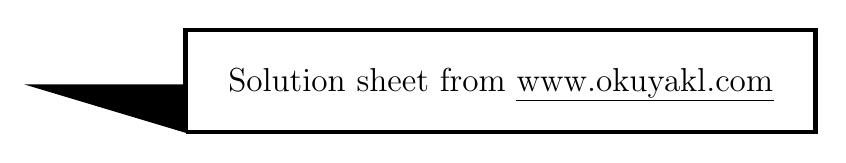
\begin{tikzpicture}(10,3)
		\draw[ultra thick](2,0) --(10,0) -- (10,1.3) --(2,1.3) -- (2,0);
		\draw[fill=black](2,0)-- (0,.6) -- (2,.6) -- (2,0);
		\node at (6,.6) {\large Solution sheet from \href{http://www.okuyakl.com}{www.okuyakl.com}};
	\end{tikzpicture}
	\vspace{0.5 cm}
	
	\noindent{\bf Task 1.}\\
	We first calculate $r$:
	$$A={ b \cdot r\over 2} \quad \Rightarrow \quad r = { 2A \over b }= {2\cdot \SI{12.5}{\centi \meter^2} \over \SI{8}{\centi\meter}}=\SI{3.125}{\centi\meter}$$
	The following also applies to the center angle:
	$$b={\mu \over 180^{\circ}}\cdot \pi r \quad \Rightarrow \quad \mu = {180^{\circ}\cdot b \over \pi r} = 147^\circ$$
	
	\noindent{\bf Task 2.}\\
	The area is a quarter circle with radius $a$ minus a semicircle with radius $a/2$:
	$$A={1\over 4} \cdot \pi a^2-{1\over 2} \cdot \pi \left({a\over 2}\right)^2 = {1\over 8}\ cdot \pi a^2 ={1\over 8}\cdot \pi \cdot (\SI{5}{\centi\meter})^2 = \SI{9.82}{\centi\meter^2} $$
	The circumference consists of the circumference of a semicircle with radius $a/2$, the circumference of a quarter circle with radius $a$ and the length $a$:
	$$U= \pi \cdot {a\over 2} + {\pi \over 2} \cdot a + a = \pi \cdot a + a = \SI{20,7}{\centi\meter}$$
	
	\noindent{\bf Task 3.}\\
	We break the figure down into subfigures:
	\begin{itemize}
		\item 2 semicircles with radius $a$; Area $A_{HK}$
		\item a square with side length $2a$; Area $A_{Q}$
		\item a triangle with base $2a$ and height $a$; Area $A_{Dr}$
	\end{itemize}
	The areas of the partial figures are added:
	$$A_{ges}=2\cdot A_{HK} + A_{Q} + A_{Dr} = 2\cdot {1\over 2} \pi a^2 + 4a^2 + {1\over 2} \cdot 2 a\cdot a = \pi a^2 + 5a^2 = a^2(5+\pi)$$
	
	\noindent
	\fbox{
		\begin{minipage}{0.47\textwidth}
			\noindent {\bf Task 4. i)}\\
			$$\alpha_{RAD}={225^\circ \over 180^\circ}\cdot \pi ={5\over 4}\pi$$
		\end{minipage}
	}
	\fbox{
		\begin{minipage}{0.47\textwidth}
			\noindent {\bf Task 4. ii)}\\
			$$\alpha_{RAD}={100^\circ \over 180^\circ}\cdot \pi ={5\over 9}\pi$$
		\end{minipage}
	}
	\fbox{
		\begin{minipage}{0.47\textwidth}
			\noindent {\bf task 4. iii)}\\
			$$\alpha_{DEG}=0.8 \cdot {180^\circ \over \pi} = 45.84^\circ$$
		\end{minipage}
	}
	\fbox{
		\begin{minipage}{0.47\textwidth}
			\noindent {\bf task 4. iv)}\\
			$$\alpha_{DEG}={7\over 4}\pi \cdot {180^\circ \over \pi} = 315^\circ$$
		\end{minipage}
	}
	\vspace{0.5cm}
	
	\noindent {\bf task 5.}\\
	$$
	\renewcommand{\arraystretch}{2}
	\begin{array}{|c|c|c|c|}
		\hline
		\qquad \mu \qquad & \qquad r \qquad &\qquad b\qquad & \qquad A_S \qquad \\
		\hline
		50^\circ & \SI{2,3}{\deci\meter} & \SI{2,0}{\deci\meter} & \SI{2,3}{\deci\meter^2} \\
		\hline
		127^\circ & \SI{4.5}{\centi\meter} & \SI{10}{\centi\meter} & \SI{22.4}{\centi\meter^2}\\
		\hline
		130^\circ & \SI{8,13}{\milli\meter} & \SI{18,5}{\milli\meter} & \SI{75}{\milli\meter^2} \\
		\hline
	\end{array}
	$$
	\begin{center}
		\includegraphics[width=7 cm]{../../viecher/eendcomic.pdf}
		
		Here you can go back to the \href{https://www.okuyakl.de/math/m10kreiaL026/ae026.pdf}{task sheet}
	\end{center}
	
\end{document}